A number of example stocks were identified in the original call, i.e.  

\begin{itemize}[labelindent=\parindent,noitemsep,topsep=0pt,parsep=0pt,partopsep=0pt]
 \item Sprat in the Celtic Sea and West of Scotland Sprat (Sub-area VI \& Divisions VIIa-c and f-k)
 \item Grey gurnard VI \& VII (excl. VIId)
 \item Ling IIIa, IVa, VI, VII, VIII, IX, XII, and XIV 
 \item Rays, primarily in areas VIIa,f,g 
 \item John dory in ICES Sub-area VII and Divisions VIIIa,b and d (Northeast Atlantic)
 \item In collaboration with Newport STO:
\begin{itemize} 
 \item Saithe VII, VIII, IX, X
 \item Pollock VII
\end{itemize}
\item Turbot VIIe,f,j,h and sub area VIII and IXa
\item Brill VII (or suitably defined)
\end{itemize}

~\newline
Available data sources and relevant publications were reviewed (Table \ref{tab:stocks}). Following which the final choice of case studies was then made in liaison with the Marine Instute based on economic value of the stock; importance of the species to the ecosystem (key-stone species); sensitivity to the impacts of fishing and available data.  

\begin{table}[h!]\centering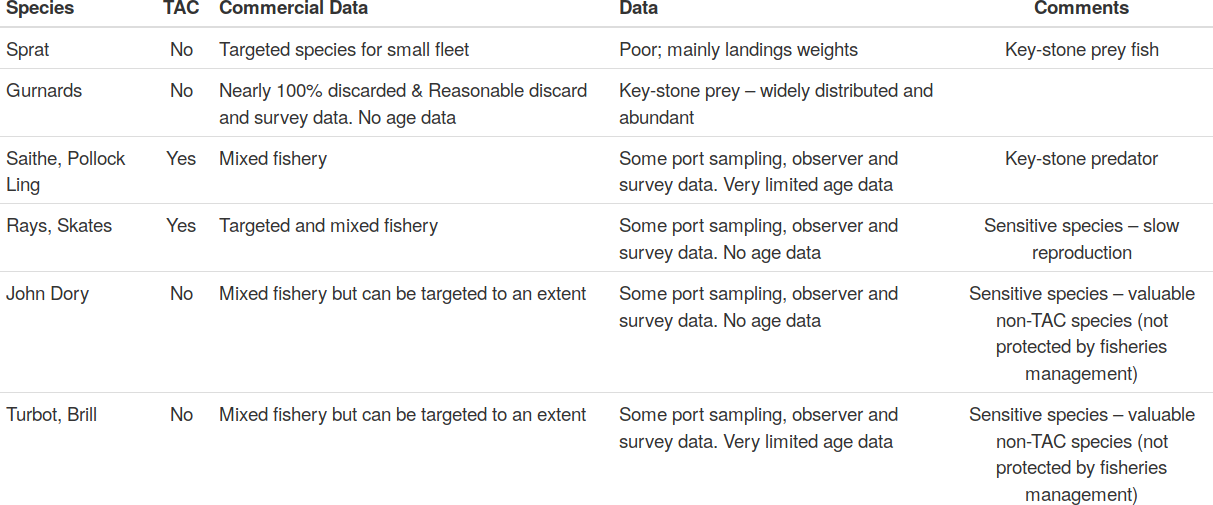
\includegraphics[width=6in]{tabs/stocks.png}\caption{Summary of potential study stocks.}\label{tab:stocks}
\end{table}
 
 
The final case studies were 
\href{https://3o2y9wugzp1kfxr5hvzgzq-on.drv.tw/MyDas/tasks/2/sprat.html}{sprat}, 
\href{https://3o2y9wugzp1kfxr5hvzgzq-on.drv.tw/MyDas/tasks/2/pollack.html}{pollack}, 
\href{https://3o2y9wugzp1kfxr5hvzgzq-on.drv.tw/MyDas/tasks/2/brill.html}{brill}, 
\href{https://3o2y9wugzp1kfxr5hvzgzq-on.drv.tw/MyDas/tasks/2/turbot.html}{turbot}, 
\href{https://3o2y9wugzp1kfxr5hvzgzq-on.drv.tw/MyDas/tasks/2/ray.html}{thornback ray}, 
\href{https://3o2y9wugzp1kfxr5hvzgzq-on.drv.tw/MyDas/tasks/2/lobster.html}{lobster} and 
\href{https://3o2y9wugzp1kfxr5hvzgzq-on.drv.tw/MyDas/tasks/2/razor.html}{razor clams} as these represent a range of life histories, and have a variety of roles in maintaining the structure of pelagic and demersal communities. The data on vertebrate life histories were accessed directly from \href{https://3o2y9wugzp1kfxr5hvzgzq-on.drv.tw/MyDas/tasks/1/stocks.html}{fishnets}. 

\begin{figure*}[h!]\centering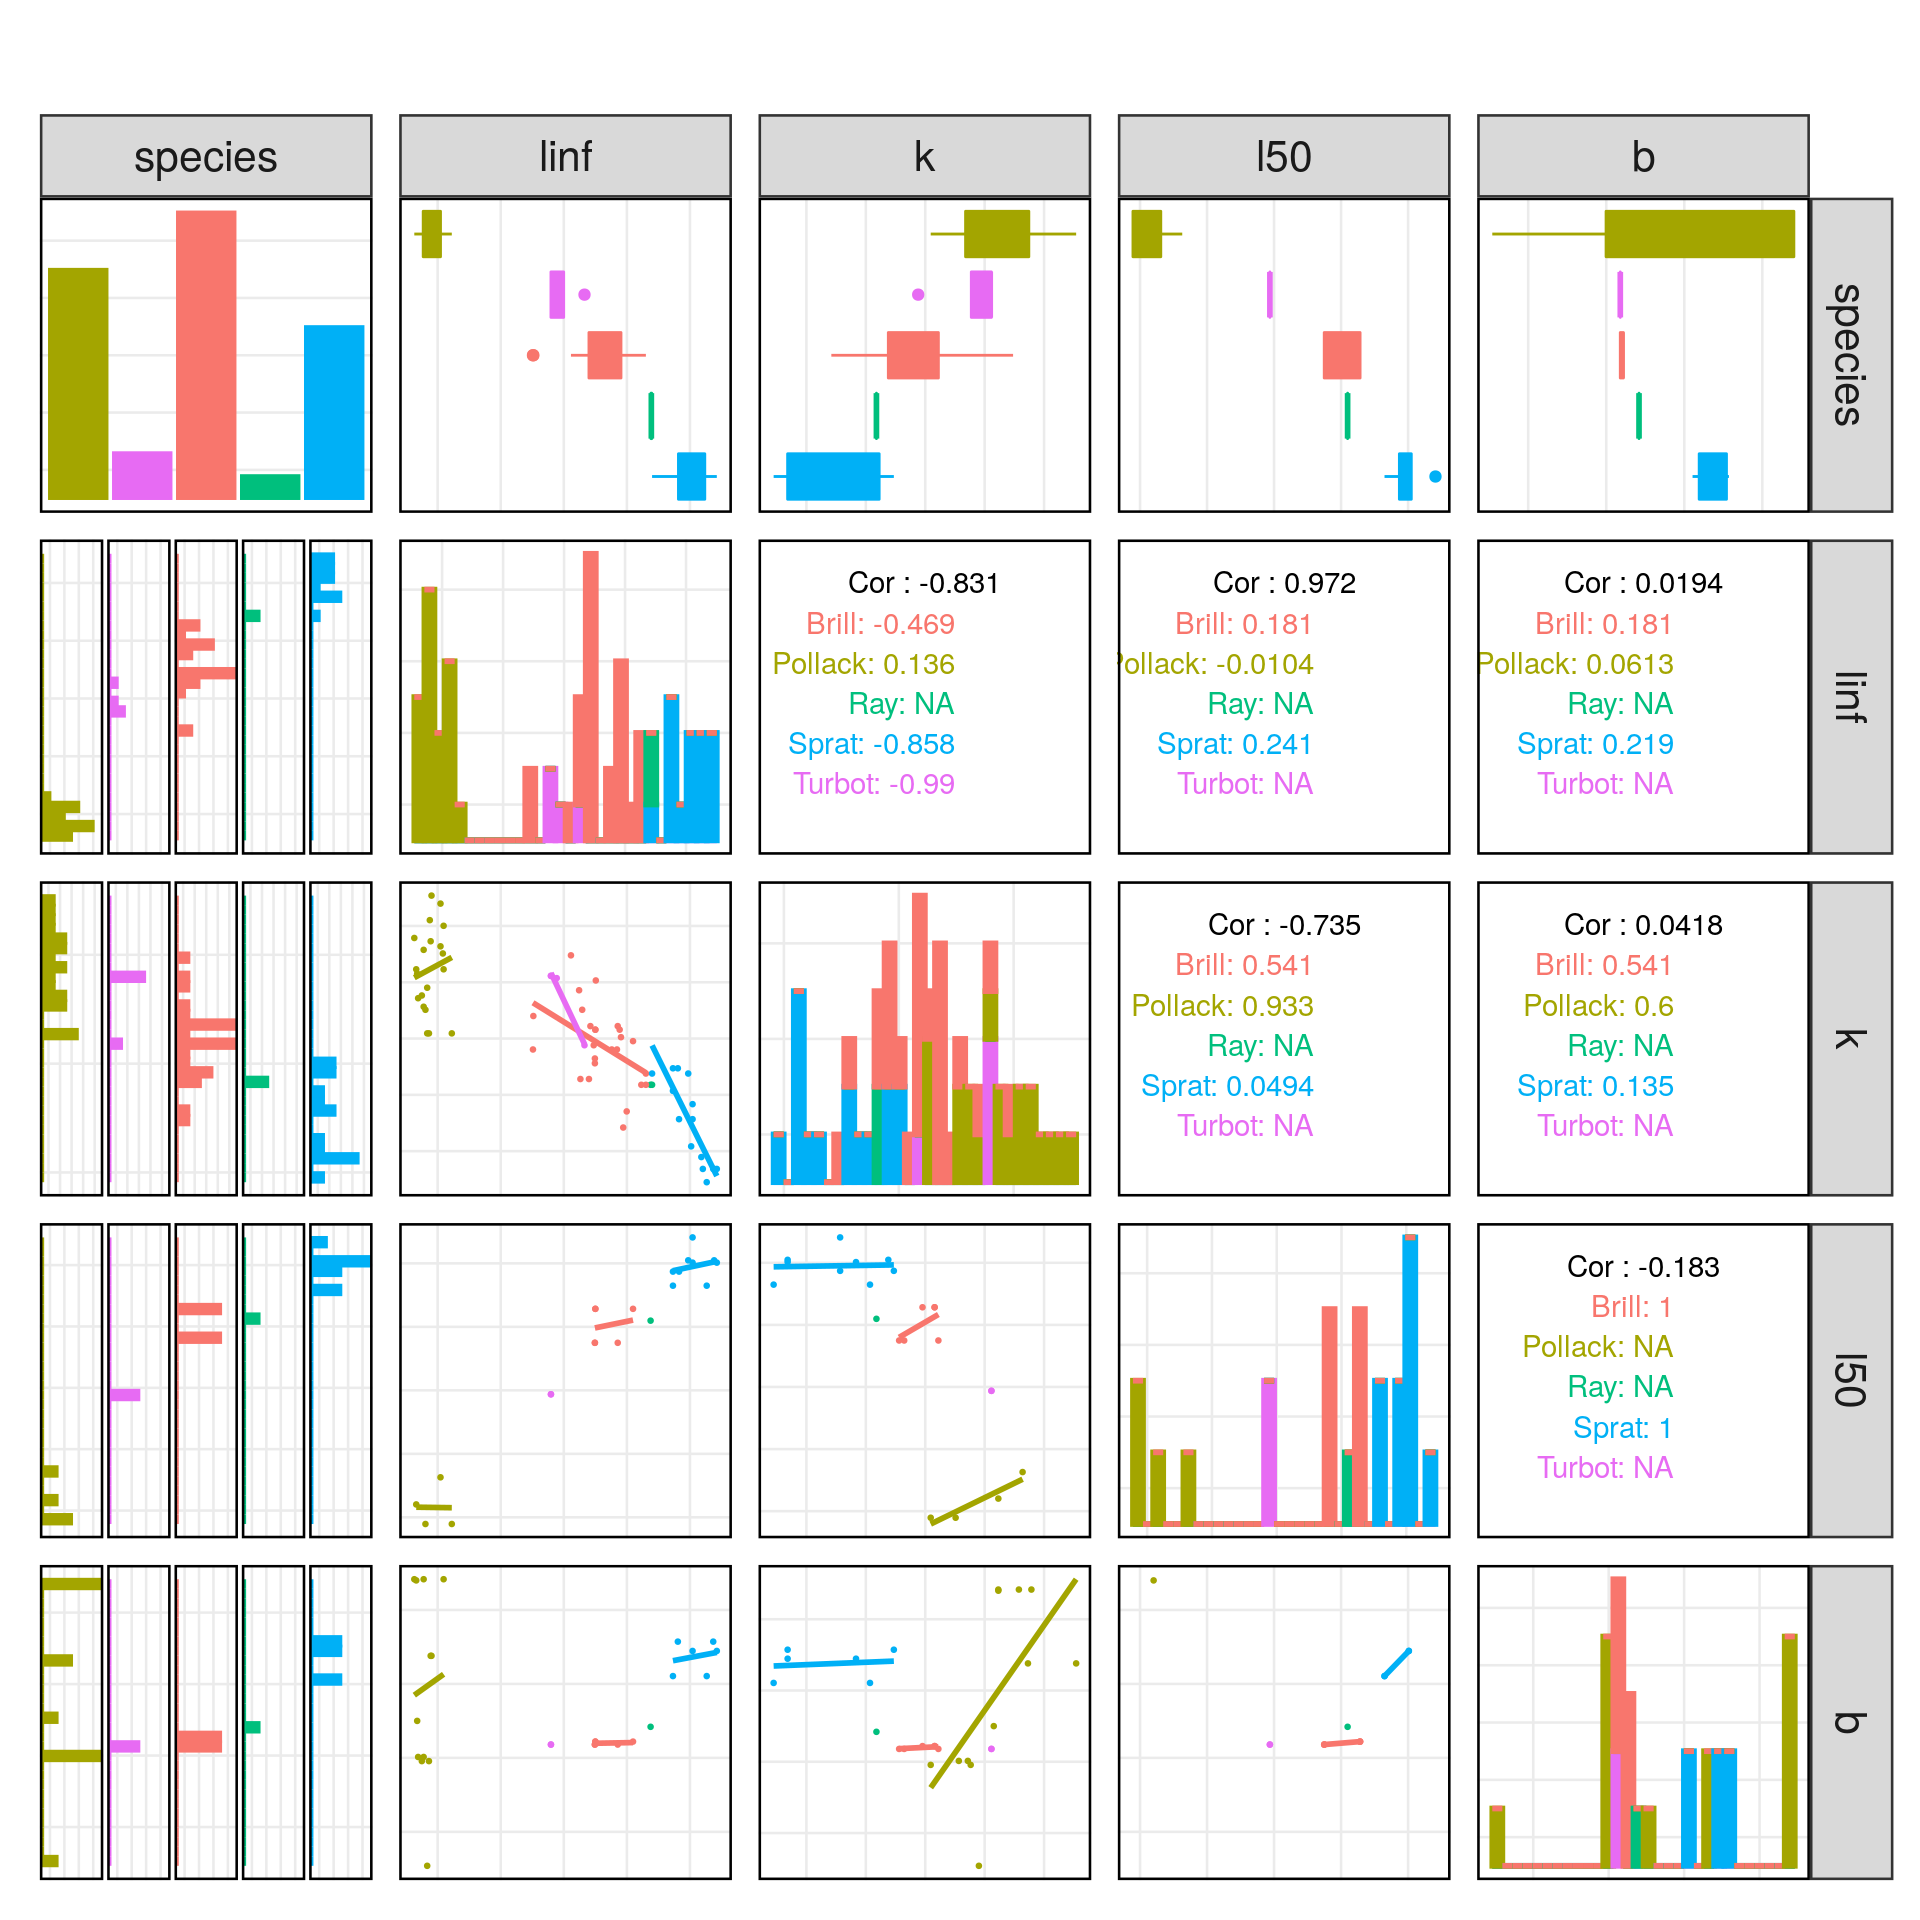
\includegraphics[width=6in]{figs/1-pairwise-1.png}\caption{Life history parameters for case study vertebrate stocks.}\label{fig:stocks}
\end{figure*}

